\chapter{Capturas de la aplicación en funcionamiento}
\label{chap:capturas}

\lettrine{E}{ste} apéndice presenta una serie de capturas que documentan el funcionamiento de la aplicación de realidad aumentada desarrollada bajo diferentes condiciones de operación. Las imágenes muestran el pipeline completo de procesamiento, desde la captura original de la cámara hasta el renderizado final del modelo 3D.

\section{Escenario sin obstrucciones}
\label{sec:unobstructed}

En este escenario el marcador cúbico se encuentra completamente visible y orientado de forma frontal respecto a la cámara. Este caso representa las condiciones ideales de funcionamiento del sistema.

\begin{figure}[H]
	\centering
	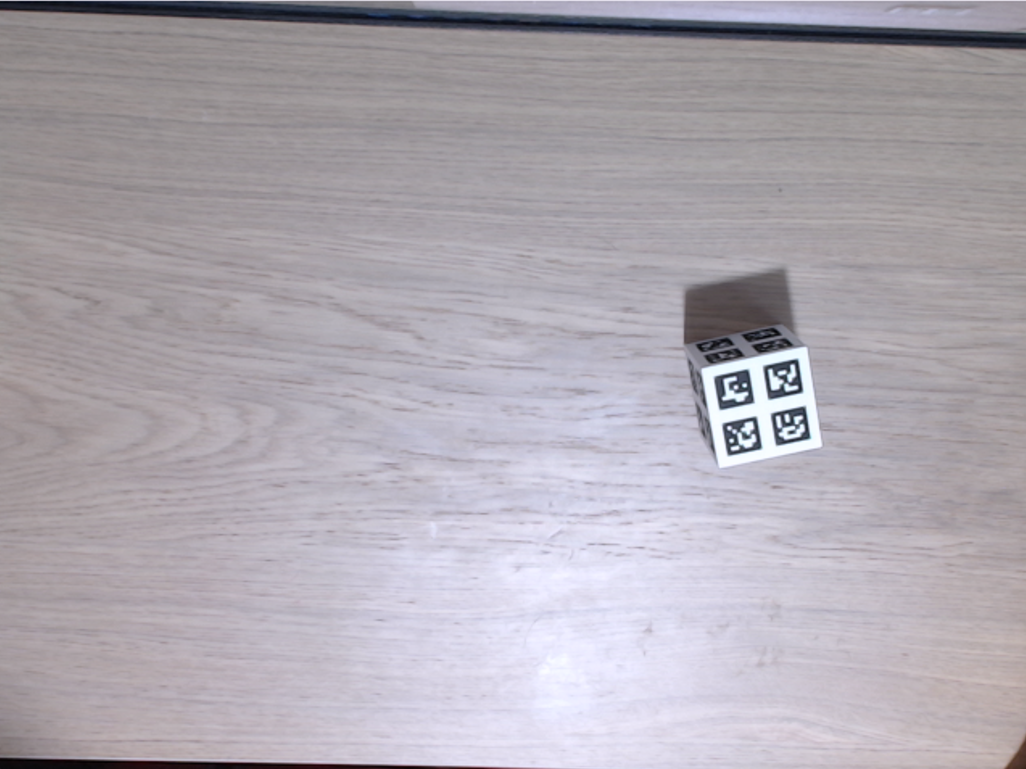
\includegraphics[width=0.8\textwidth]{imaxes/unobstructed_raw_image.png}
	\caption{Imagen original.}
	\label{fig:unobstructed_raw}
\end{figure}

\begin{figure}[H]
	\centering
	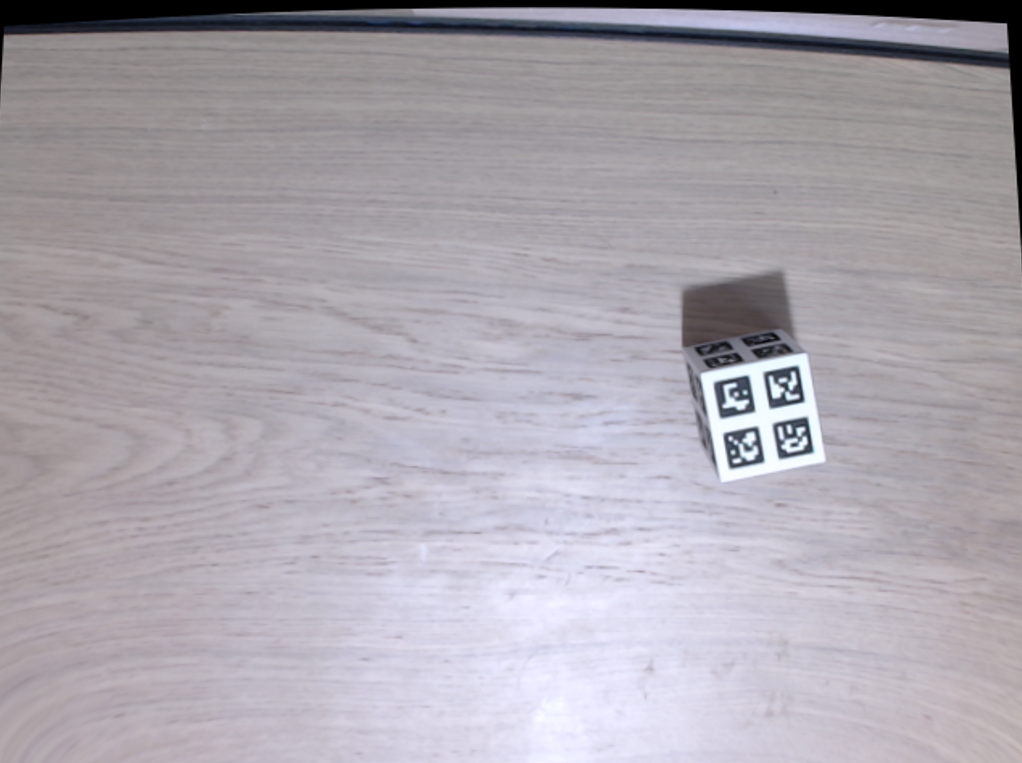
\includegraphics[width=0.8\textwidth]{imaxes/unobstructed_undistorted.png}
	\caption{Imagen corregida tras aplicar la corrección de distorsión de la cámara.}
	\label{fig:unobstructed_undistorted}
\end{figure}

\begin{figure}[H]
	\centering
	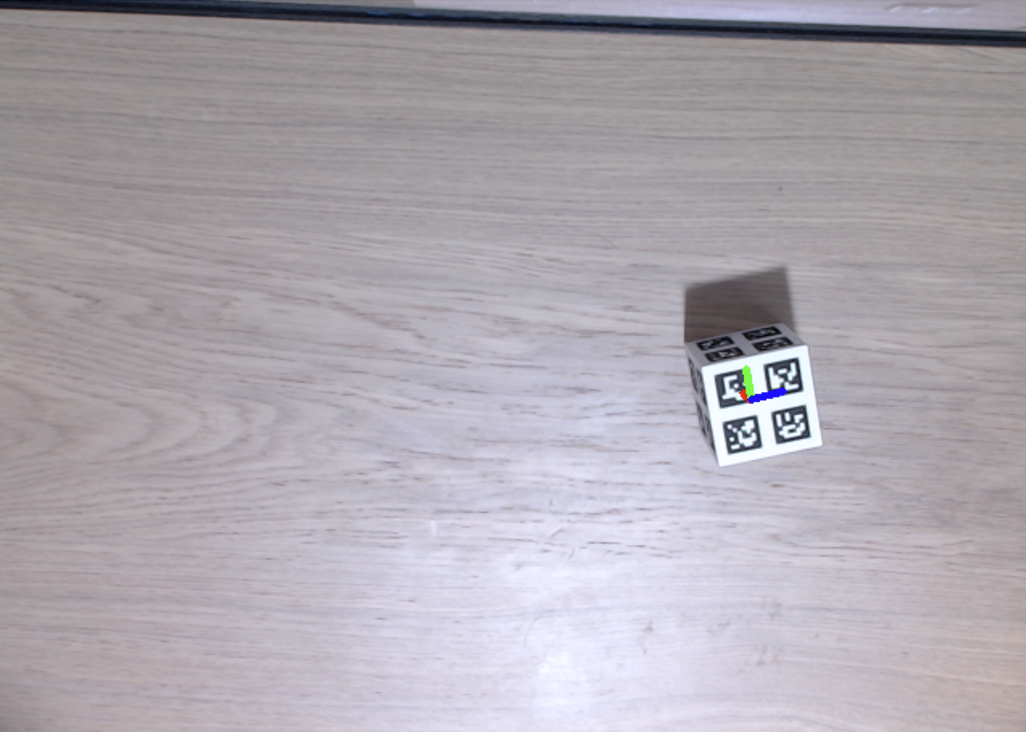
\includegraphics[width=0.8\textwidth]{imaxes/unobstructed_cube_axis.png}
	\caption{Visualización de los ejes de coordenadas sobre el marcador detectado.}
	\label{fig:unobstructed_axes}
\end{figure}

\begin{figure}[H]
	\centering
	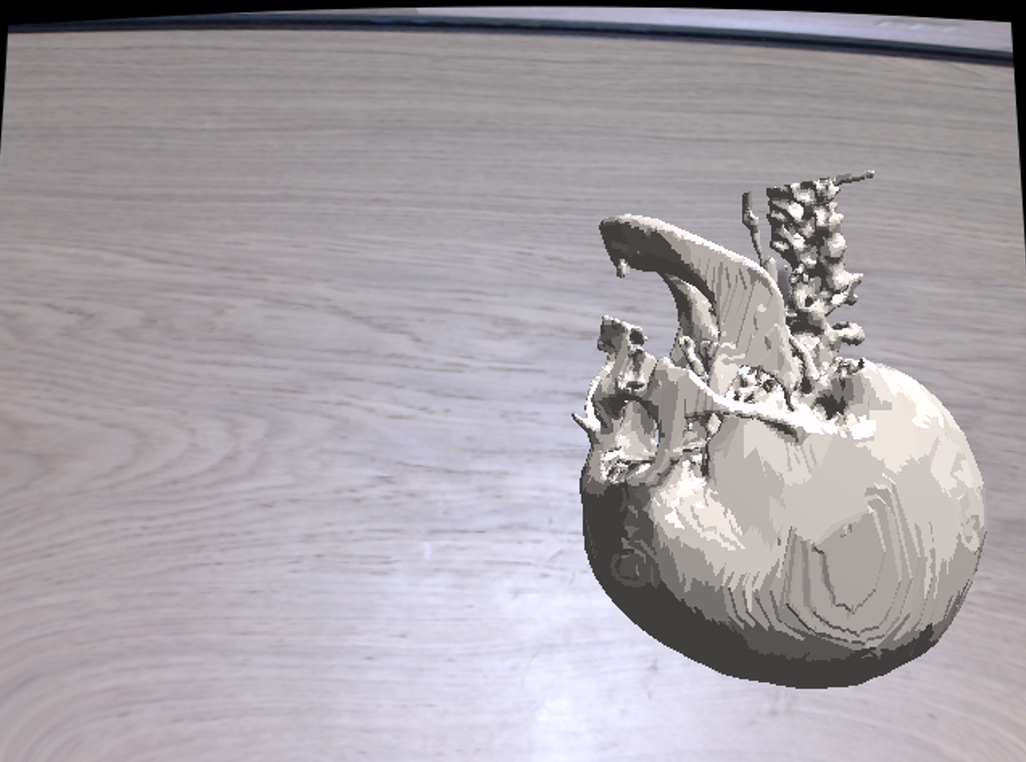
\includegraphics[width=0.8\textwidth]{imaxes/unobstructed_opengl_render.png}
	\caption{Renderizado final del modelo 3D.}
	\label{fig:unobstructed_render}
\end{figure}

\section{Escenario con inclinación}
\label{sec:tilted}

Este escenario evalúa el comportamiento del sistema cuando varias caras del marcador son detectadas.

\begin{figure}[H]
	\centering
	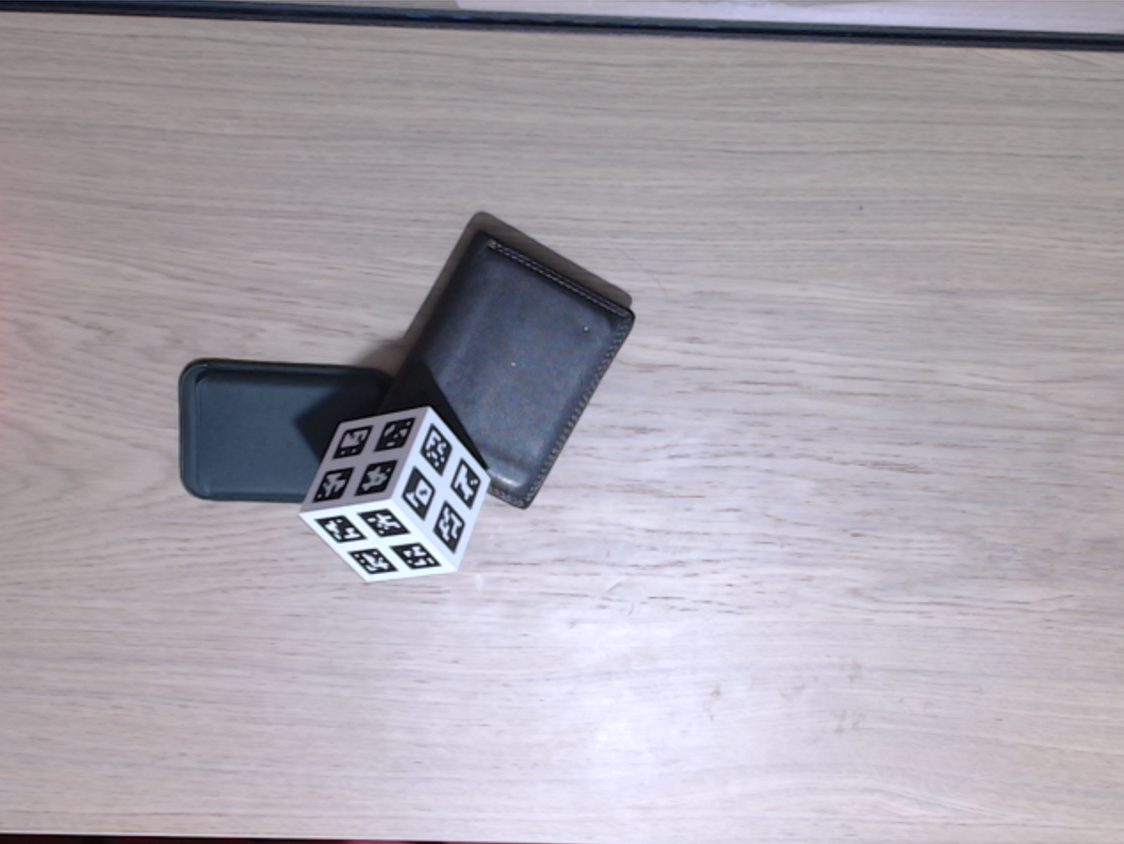
\includegraphics[width=0.8\textwidth]{imaxes/tilted_raw_image.png}
	\caption{Imagen original del marcador inclinado.}
	\label{fig:tilted_raw}
\end{figure}

\begin{figure}[H]
	\centering
	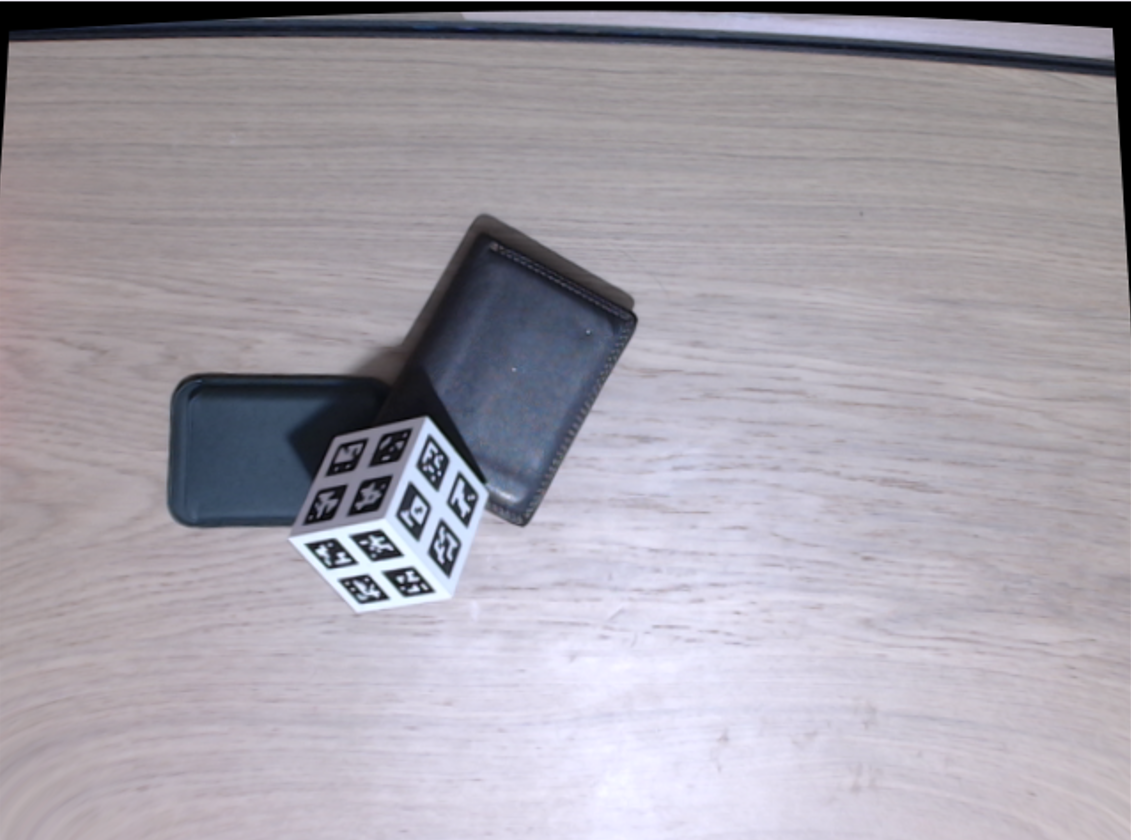
\includegraphics[width=0.8\textwidth]{imaxes/tilted_undistorted.png}
	\caption{Imagen corregida del marcador.}
	\label{fig:tilted_undistorted}
\end{figure}

\begin{figure}[H]
	\centering
	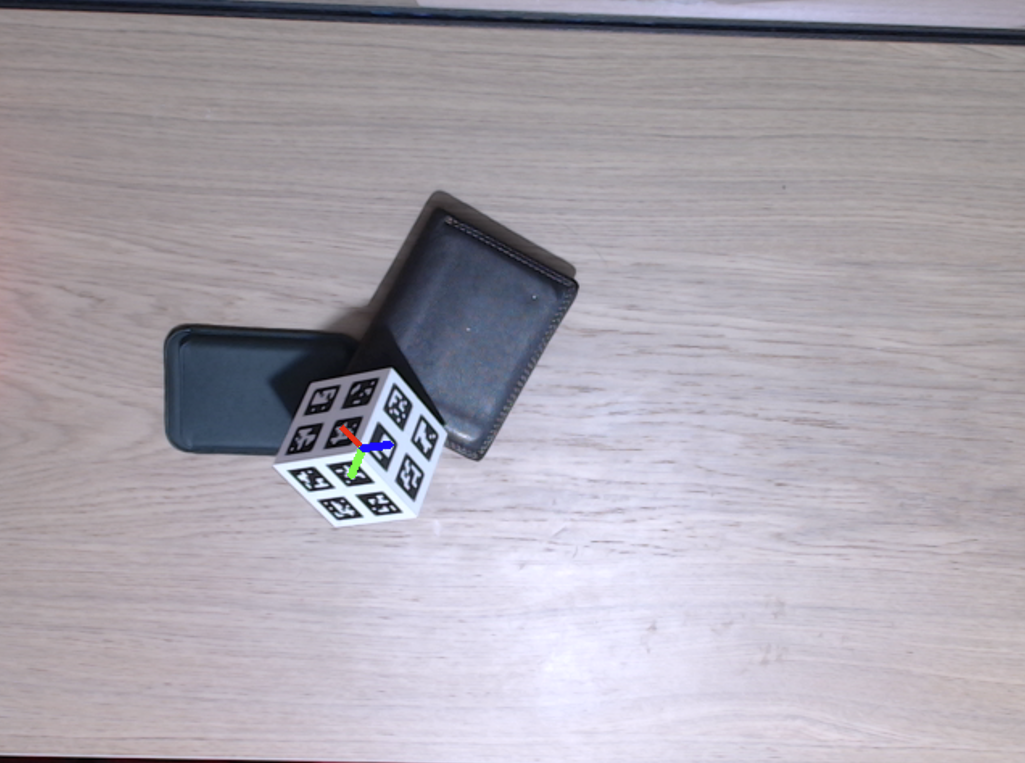
\includegraphics[width=0.8\textwidth]{imaxes/tilted_cube_axis.png}
	\caption{Ejes de coordenadas renderizados sobre el marcador.}
	\label{fig:tilted_axes}
\end{figure}

\begin{figure}[H]
	\centering
	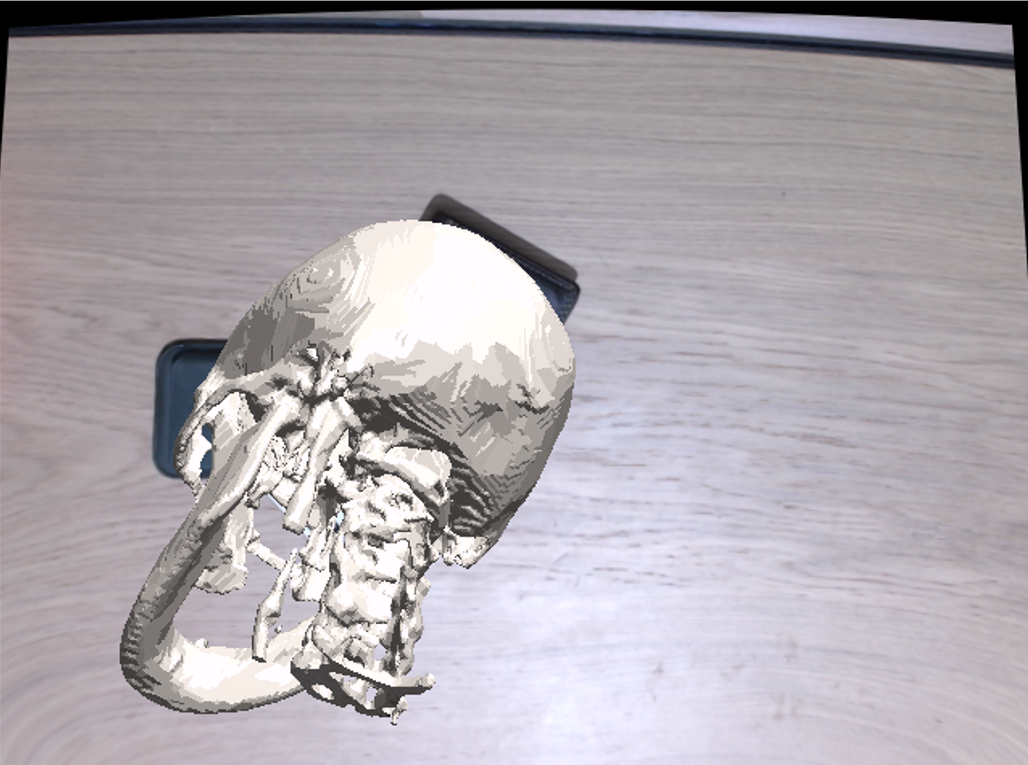
\includegraphics[width=0.8\textwidth]{imaxes/tilted_opengl_render.png}
	\caption{Modelo 3D renderizado sobre el marcador.}
	\label{fig:tilted_render}
\end{figure}

\section{Escenario con oclusión parcial}
\label{sec:ocluded}

En este escenario se evalúa la capacidad del sistema para mantener el seguimiento cuando parte del marcador cúbico está oculto.

\begin{figure}[H]
	\centering
	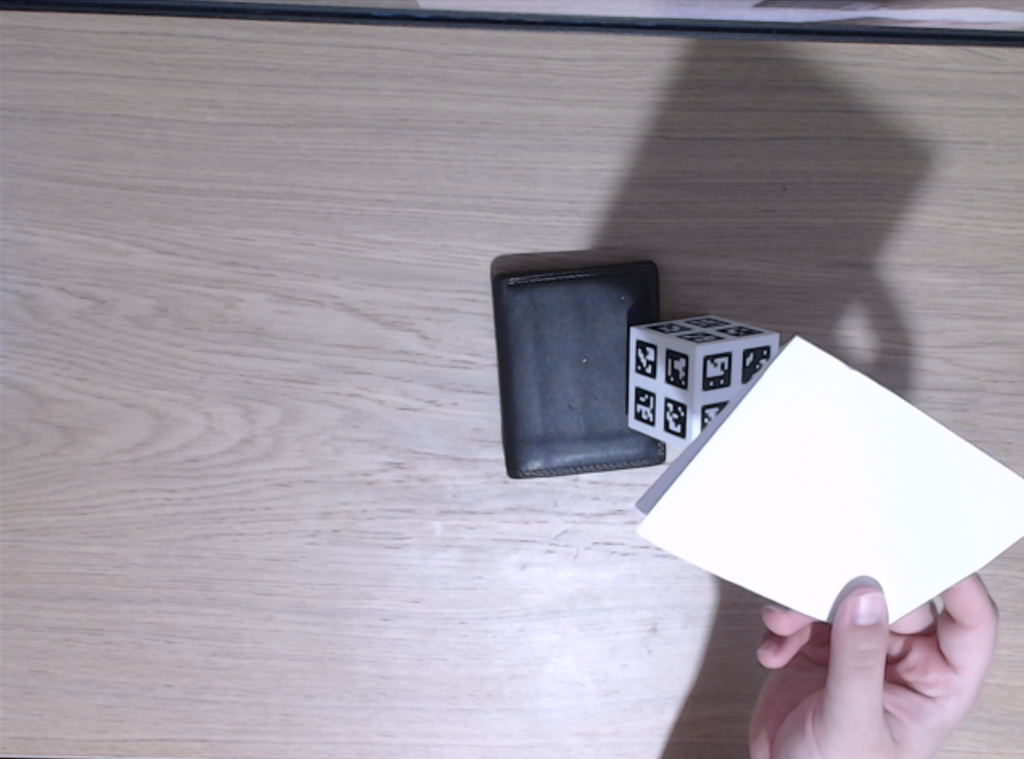
\includegraphics[width=0.8\textwidth]{imaxes/ocluded_raw_image.png}
	\caption{Imagen original del marcador con oclusión parcial.}
	\label{fig:ocluded_raw}
\end{figure}

\begin{figure}[H]
	\centering
	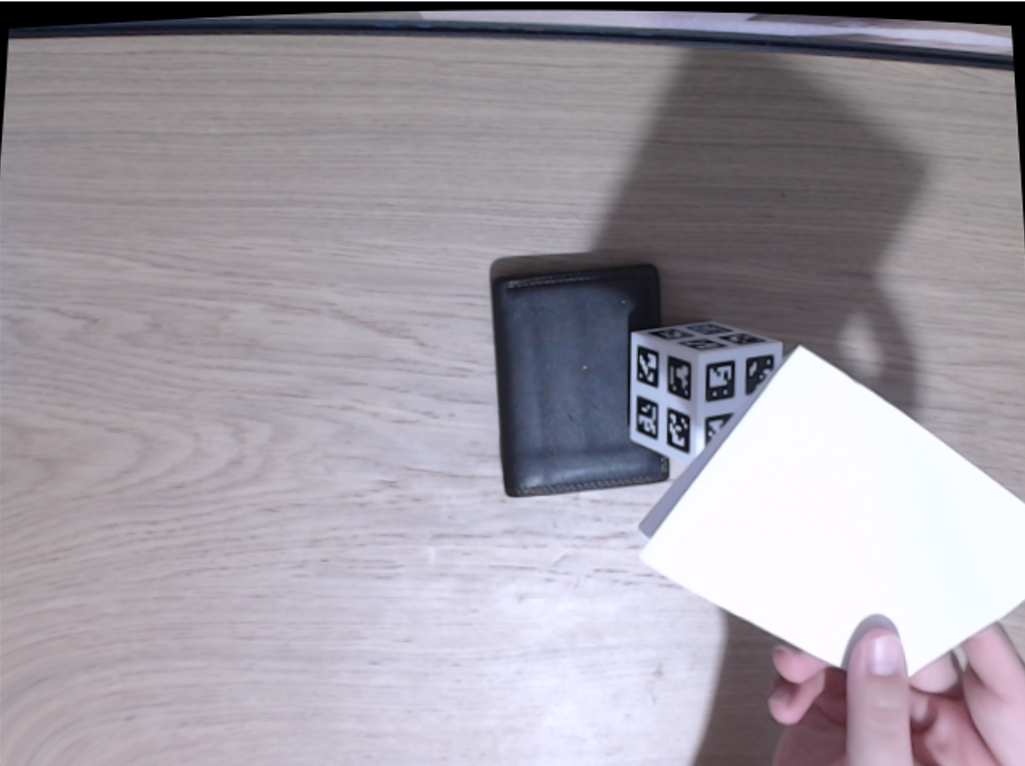
\includegraphics[width=0.8\textwidth]{imaxes/ocluded_undistorted.png}
	\caption{Imagen corregida del marcador ocluido tras la corrección de distorsión.}
	\label{fig:ocluded_undistorted}
\end{figure}

\begin{figure}[H]
	\centering
	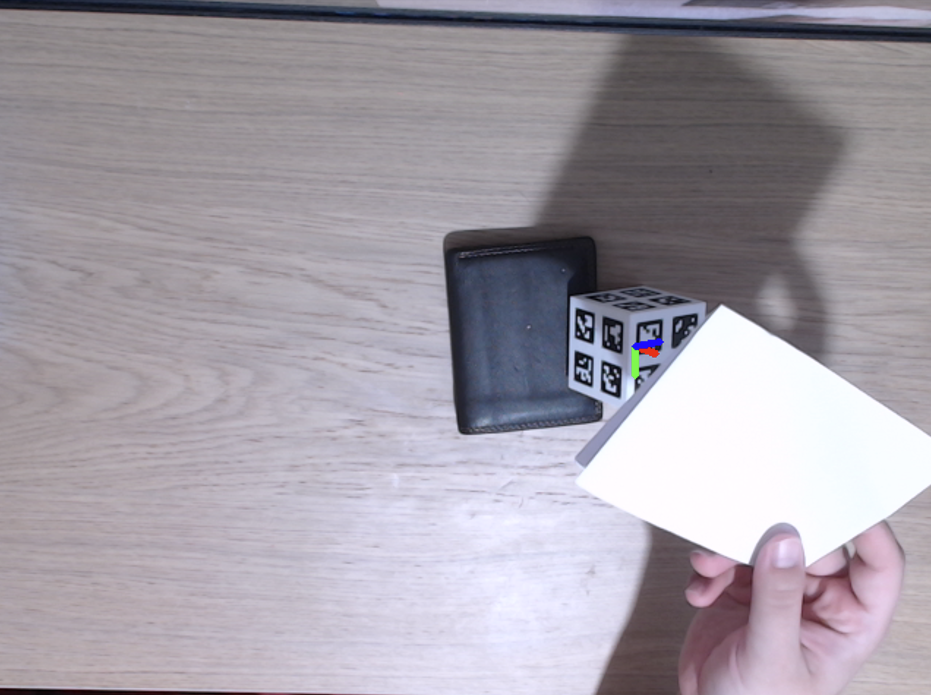
\includegraphics[width=0.8\textwidth]{imaxes/ocluded_cube_axis.png}
	\caption{Ejes de coordenadas renderizados sobre el marcador parcialmente ocluido.}
	\label{fig:ocluded_axes}
\end{figure}

\begin{figure}[H]
	\centering
	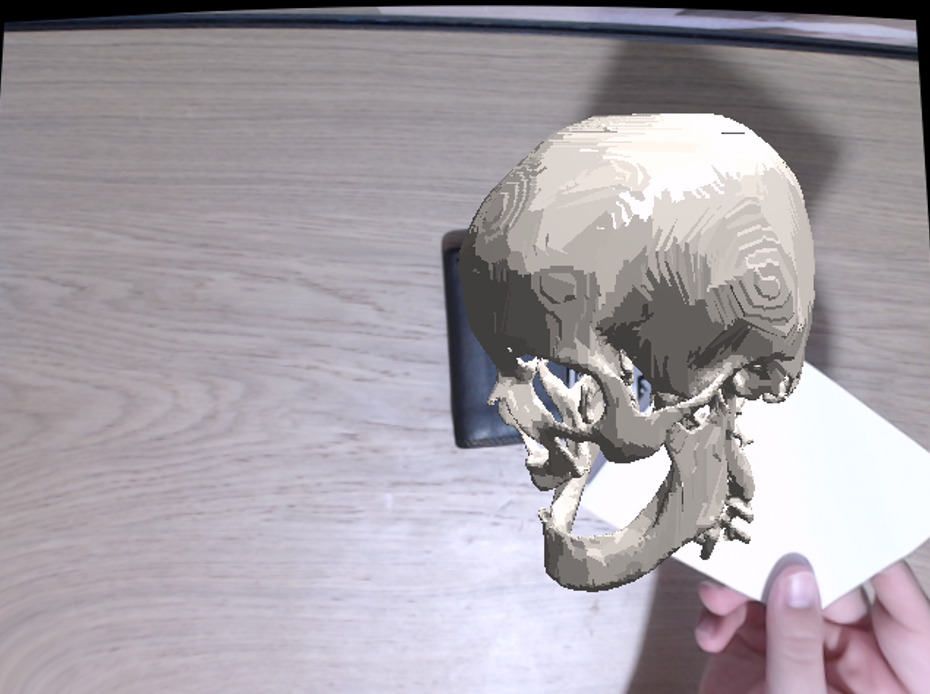
\includegraphics[width=0.8\textwidth]{imaxes/ocluded_opengl_render.png}
	\caption{Modelo 3D renderizado sobre el marcador.}
	\label{fig:ocluded_render}
\end{figure}